\documentclass[tikz,border=6pt]{standalone}
\usepackage[T1]{fontenc}
\usepackage{lmodern}
\usepackage{amsmath,amssymb}
\usetikzlibrary{positioning,arrows.meta,fit,calc}
% Design of koblitz-n83-closure-20261019 (frozen protocol.json). Not a result.
\begin{document}
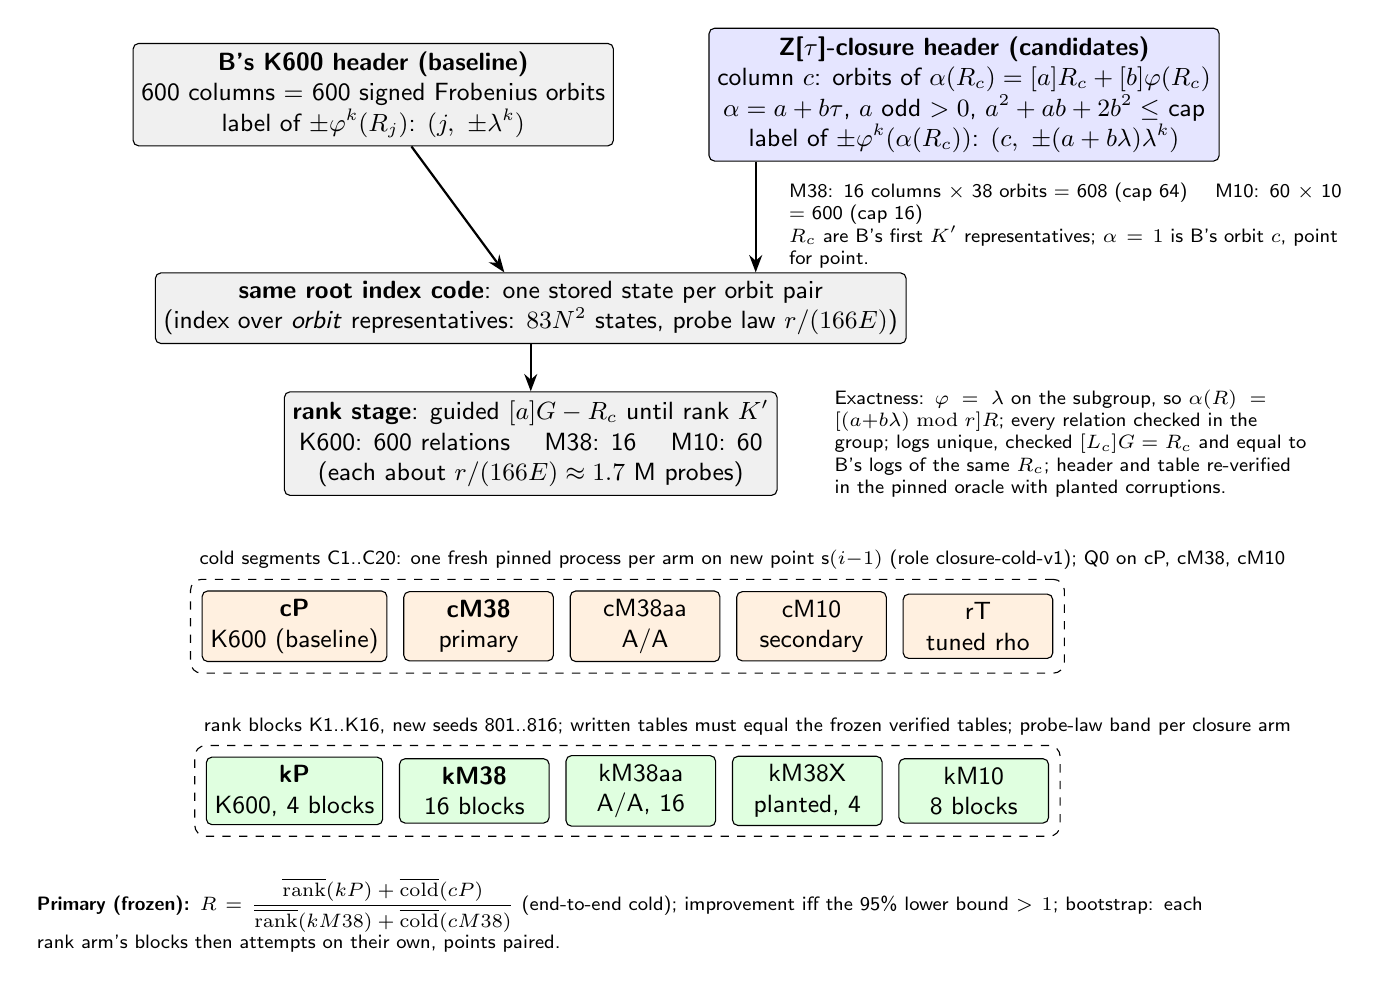
\begin{tikzpicture}[
  font=\sffamily\small,
  box/.style={draw, rounded corners=2pt, align=center, minimum height=8mm, inner sep=3pt},
  base/.style={box, fill=gray!12},
  add/.style={box, fill=blue!10},
  arm/.style={box, fill=orange!12, minimum width=19mm},
  rank/.style={box, fill=green!12, minimum width=19mm},
  arr/.style={-{Stealth[length=2.2mm]}, thick},
  note/.style={align=left, font=\sffamily\scriptsize}
]
\node[base] (b) {\textbf{B's K600 header (baseline)}\\600 columns = 600 signed Frobenius orbits\\label of $\pm\varphi^k(R_j)$: $(j,\ \pm\lambda^k)$};
\node[add, right=12mm of b] (c) {\textbf{Z[$\tau$]-closure header (candidates)}\\column $c$: orbits of $\alpha(R_c)=[a]R_c+[b]\varphi(R_c)$\\$\alpha=a+b\tau$, $a$ odd $>0$, $a^2+ab+2b^2\le$ cap\\label of $\pm\varphi^k(\alpha(R_c))$: $(c,\ \pm(a+b\lambda)\lambda^k)$};
\node[note, anchor=north west, text width=72mm] (cn) at ($(c.south west)+(9mm,-1.5mm)$) {M38: 16 columns $\times$ 38 orbits = 608 (cap 64) \quad M10: 60 $\times$ 10 = 600 (cap 16)\\
$R_c$ are B's first $K'$ representatives; $\alpha=1$ is B's orbit $c$, point for point.};
\node[base, below=16mm of b, xshift=20mm] (idx) {\textbf{same root index code}: one stored state per orbit pair\\(index over \emph{orbit} representatives: $83N^2$ states, probe law $r/(166E)$)};
\draw[arr] (b) -- (idx); \coordinate (s) at ($(c.south west)+(6mm,0)$); \draw[arr] (s) -- (s |- idx.north);
\node[base, below=6mm of idx] (rk) {\textbf{rank stage}: guided $[a]G-R_c$ until rank $K'$\\K600: 600 relations \quad M38: 16 \quad M10: 60\\(each about $r/(166E)\approx1.7$ M probes)};
\draw[arr] (idx) -- (rk);
\node[note, right=6mm of rk, text width=60mm] {Exactness: $\varphi=\lambda$ on the subgroup, so $\alpha(R)=[(a{+}b\lambda)\bmod r]R$;
every relation checked in the group; logs unique, checked $[L_c]G=R_c$ and equal to B's logs of the same $R_c$; header and table re-verified in the pinned oracle with planted corruptions.};
% Cold arms
\node[arm, below=12mm of rk, xshift=-30mm] (cP) {\textbf{cP}\\K600 (baseline)};
\node[arm, right=2mm of cP] (cM) {\textbf{cM38}\\primary};
\node[arm, right=2mm of cM] (cMa) {cM38aa\\A/A};
\node[arm, right=2mm of cMa] (cT) {cM10\\secondary};
\node[arm, right=2mm of cT] (rT) {rT\\tuned rho};
\node[draw, dashed, rounded corners, fit=(cP) (rT), inner sep=4pt, label={[note, anchor=south west]north west:{cold segments C1..C20: one fresh pinned process per arm on new point s$(i{-}1)$ (role closure-cold-v1); Q0 on cP, cM38, cM10}}] (cold) {};
\node[rank, below=12mm of cP] (kP) {\textbf{kP}\\K600, 4 blocks};
\node[rank, right=2mm of kP] (kM) {\textbf{kM38}\\16 blocks};
\node[rank, right=2mm of kM] (kMa) {kM38aa\\A/A, 16};
\node[rank, right=2mm of kMa] (kMX) {kM38X\\planted, 4};
\node[rank, right=2mm of kMX] (kT) {kM10\\8 blocks};
\node[draw, dashed, rounded corners, fit=(kP) (kT), inner sep=4pt, label={[note, anchor=south west]north west:{rank blocks K1..K16, new seeds 801..816; written tables must equal the frozen verified tables; probe-law band per closure arm}}] (rkb) {};
\node[note, below=4mm of rkb, text width=150mm] {\textbf{Primary (frozen):}
$R=\dfrac{\overline{\mathrm{rank}}(kP)+\overline{\mathrm{cold}}(cP)}{\overline{\mathrm{rank}}(kM38)+\overline{\mathrm{cold}}(cM38)}$ (end-to-end cold);
improvement iff the 95\% lower bound $>1$; bootstrap: each rank arm's blocks then attempts on their own, points paired.};
\end{tikzpicture}
\end{document}
